\documentclass[12pt, letterpaper, twoside]{article}
\usepackage[utf8]{inputenc}
\usepackage{titlesec}
% Minted package is used for the command line samples provided in the document
\usepackage{minted}
\usepackage{graphicx}
\graphicspath{ {./} }

\newcommand{\sectionbreak}{\clearpage}

% removes the red box from the dollar sign that comes by default with minted.
\AtBeginEnvironment{minted}{\dontdofcolorbox}
\def\dontdofcolorbox{\renewcommand\fcolorbox[4][]{##4}}

\title{
    \textbf{Info-Mine}\\
    {Software lab project}\\
    {INDIAN INSTITUTE OF TECHNOLOGY, BOMBAY}
}
\author{ 
    \textbf{Rohit Kundu}\\203050030\\
    \textbf{Pranshu Chourasia}\\203050098\\
    \textbf{Raghunath Das}\\203050071\\
    \textbf{Pramod S Rao}\\20305R007\\
}

\date{18th November, 2020}

\begin{document}
\maketitle

\tableofcontents

\section{Introduction}
    The info-mine project aims at bringing together the information spread across various locations at IIT-B into one spot
    for a user to be able to access information faster and cleaner. As of now, when a student wants to get any information, from the cse website, their emails, or moodle, they login to each of the portals and then look for the information. Also, sometimes, a student can miss out on some announcements and due dates. Info-Mine helps to gather all of this information and provide it to the student as a command line tool for linux users and also a whatsapp bot for non-linux users, where they can just type a command and information will be fetched for them.\\
    For the command line tool, in the CSE component, we fetch information from the cse website regarding students, faculties, news and courses. In the moodle component we fetch all sorts of information for a student, like quizzes, grades, assignments, announcements, discussions, courses and forums. We also have a component which will send and retrieve emails with simple commands, instead of logging in to see one email, we can just send a simple command to fetch the email for us, or even filter multiple emails directly from the command line. All of these components are also made available on Whatsapp for students who do not use the terminal. 

    \subsection{Motivation}
        Many of the courses tend to prefer certain platforms over the others for providing updates, quiz info, discussions etc. 
        Also, apart from the courses, we have two emails, which are institute and department mails.
        This causes a student to visit multiple sites many times which can get discomforting after a certain point, and this can cause students to miss out on some updates. 
        Thus, the aim of this project is to reduce the hindrance in visting many places and create a tool that helps students to get all their info
        in one spot. The term Info-Mine comes from mining for information from cse websites, moodle and the emails.
        
    \subsection{Installation}
        There are two ways to use this, via a linux command line, or through whatsapp. \\ 
        \\
        For the installation of the command line tool, perform the following:
        \begin{itemize}
            \item cd into the directory that you want to install this tool.
            \item To download the installer to this directory, on your command line perform: \textbf{wget --no-check-certificate --content-disposition https://raw.githubusercontent.com/RKKUNDU/info-mine/main/infomine-installer.sh}
            \item Run the installer script with root priviliges, by: \textbf{sudo bash infomine-installer.sh}
            \item Now you will be able to run 'infomine' from anywhere within your system.
            \item Please read the remaining sections to perform the commands.
        \end{itemize} 
        To register for whatsapp, perform the following:
        \begin{itemize}
            \item Please go to \textbf{http://infomine.pythonanywhere.com/}
            \item Enter the mentioned details.
            \item You will receive instructions upon what to do next.
            \item The instructions will mostly comprise of sending a certain message to a number on Whatsapp.
            \item Please read the remaining sections to perform the commands.
        \end{itemize}

\section{Moodle}
When using the moodle component of info-mine, they will have to provide their userid and password over command prompt.
A user will be prompted for these details only when using it for the first time and these details are encrypted and stored in the configs
folder. 
These credentials are then used to make the subsequent requests.
A user can then fetch 7 types of information from their moodle website, details of which are mentioned in the below subsections.
To find more info from the command line the user can simply perform the below command
\begin{minted}[frame=lines, framesep=4mm, encoding=utf8]{text}
/home/user$: infomine moodle -h
usage: infomine moodle [-h] {quizzes,grades,forums,discussions,
courses,announcements,assignments} ...
positional arguments:
{quizzes,grades,forums,discussions,courses,announcements,assignments}
                        Moodle commands help
    quizzes             Info about quizzes
    grades              Info about grades
    forums              Info about discussion forums
    discussions         Info about discussions
    courses             Info about courses
    announcements       Info about announcements
    assignments         Info about assignments

optional arguments:
-h, --help            show this help message and exit

\end{minted}
    This provides the user with seven options from which he can choose to fetch his/her data.
    Let's start with quizzes.
\subsection{Quizzes}
To get information on how to use the quizzes module, the user can do so with a -h flag like
\begin{minted}[frame=lines, framesep=4mm, encoding=utf8]{text}
/home/user$: infomine moodle quizzes -h
usage: infomine moodle quizzes [-h] [-c CID]

optional arguments:
    -h, --help         show this help message and exit
    -c CID, --cid CID  Show quizzes of given course
\end{minted}
As you can see from the usage, by providing no flags, the user will simply get a list of all the quizzes for all the courses he/she has registered.\\
To get a list of the quizzes for a particular course, we need to use the -c flag with the course id(course id is with respect to moodle and can be found from the moodle courses module) we can for example:

\begin{minted}[frame=lines, framesep=4mm]{text}
/home/user$: infomine moodle quizzes -c 222
Sl No    Course id    id Name Total Score  Quiz Opens   Quiz Closes
-------  -----------  ----  ----------------------------------------
1          222    64  Quiz 6 2020-08-13 10:30:00  2020-08-16 23:59:00
2          222   432  Quiz 7 2020-08-13 10:30:00 2020-08-16 23:59:00
\end{minted}

\subsection{Grades}
To get information on how to use the grades module, the user can do so with a -h flag like 
\begin{minted}[frame=lines, framesep=4mm, encoding=utf8]{text}
/home/user$: infomine moodle grades -h
usage: infomine moodle grades [-h] -c CID

optional arguments:
  -h, --help         show this help message and exit
  -c CID, --cid CID  Show grades of given course
\end{minted}
As you can see from the usage, by providing no flags, the user will simply get a list of all the grades for all the courses he/she has registered.\\
To get a list of the grades for a particular course, we need to use the -c flag with the course id(course id is with respect to moodle and can be found from the moodle courses module) we can for example:

\begin{minted}[frame=lines, framesep=4mm]{text}
/home/user$: infomine moodle grades -c 222
sl No      Grade    Max  Percentage
-------  ---------  -----  ------------
      1                 6  -
      2    7            9  77.78 %
      3    4.33333      6  72.22 %
    
\end{minted}

\subsection{Forums}
To get information on how to use the forums module, the user can do so with a -h flag like 
\begin{minted}[frame=lines, framesep=4mm, encoding=utf8]{text}
/home/user$: infomine moodle forums -h
usage: infomine moodle forums [-h] -c CID
                               [-n NUMBER]

optional arguments:
  -h, --help            show this help message and
                        exit
  -c CID, --cid CID     Show forums of given course
  -n NUMBER, --number NUMBER
                        Show only top n discussion
                        forums
\end{minted}
For using the forums module we need to provide -c flag and provide the course id (course id is with respect to moodle and can be found from the moodle courses module), it is mandatory. The -n flag is to provide the top number of entries we want to filter and see in the output\\
To get a list of 'n' forums for a course we can for example:

\begin{minted}[frame=lines, framesep=4mm]{text}
/home/user$: infomine moodle forums -c 224 -n 2
Forum ID  Forum Name
----------  ----------------
       223  Announcements
      1159  Discussion Forum
\end{minted}

\subsection{Discussions}
To get information on how to use the discussions module, the user can do so with a -h flag like 
\begin{minted}[frame=lines, framesep=4mm, encoding=utf8]{text}
usage: infomine moodle discussions [-h] -f FORUM_ID [-n NUMBER]

optional arguments:
    -h, --help            show this help message and exit
    -f FORUM_ID, --forum-id FORUM_ID
                        Show discussions of given forum
    -n NUMBER, --number NUMBER
                        Show only top n discussions    
\end{minted}
For using the discussions module we need to provide -f flag and provide the forum id (forum id is with respect to moodle and can be found from the moodle forums module), it is mandatory to know which forum's discussion you are trying to fetch. The -n flag is to provide the top number of entries we want to filter and see in the output\\
To get a list of 'n' discussions for a forum we can for example:

\begin{minted}[frame=lines, framesep=4mm]{text}
/home/user$: infomine moodle discussions -f 223 -n 2
Discussions:
         1. 2020-10-21 11:23:59 PA4 description posted
Check out the next programming assignment. 

         2. 2020-10-12 20:18:47 Midsem cribs
For any issues regarding the marks/solutions in midsem please fill this form.https://forms.gle/bmgAjW6SmBXPCiH48
\end{minted}

\subsection{Courses}
To get information on how to use the courses module, the user can do so with a -h flag like 
\begin{minted}[frame=lines, framesep=4mm, encoding=utf8]{text}
/home/user$: infomine moodle courses -h
usage: infomine moodle courses [-h]

optional arguments:
    -h, --help  show this help message and exit
\end{minted}
This is the simplest module to use as we don't have to pass any argument. We are simply returned a list of the courses in which we have registered.\\
Apart from courses registered, we also get important info like the course id which can be later used in the other moodle modules.
This also provides us with information on our progress made so far in the course.
Also, course code information is provided.
To get a list of courses we have registered:\\
\\
\begin{minted}[frame=lines, framesep=4mm]{text}
/home/user$: infomine moodle courses
sl No    Course id    Progress  Short Name     Full Name
-------  ----------- ----------  ------------- ----------
1  226   7.69231  CS 765-2020-1  Introduction to Blockchain
2  224   100      CS 744-2020-1  Design and Engineering of Computing Systems
3  219   88.8889  CS 699-2020-1  Software Lab.
\end{minted}

\subsection{Announcements}
To get information on how to use the announcements module, the user can do so with a -h flag like 
\begin{minted}[frame=lines, framesep=4mm, encoding=utf8]{text}
/home/user$: infomine moodle announcements -h
usage: infomine moodle announcements [-h] -c CID [-n NUMBER]

optional arguments:
  -h, --help            show this help message and exit
  -c CID, --cid CID     Show announcements of given course
  -n NUMBER, --number NUMBER
                        Show only top n announcements
\end{minted}
For using the announcements module we need to provide -c flag and provide the course id (course id is with respect to moodle and can be found from the moodle course module), it is mandatory to know which course's announcements you are trying to fetch. The -n flag is to provide the top number of entries we want to filter and see in the output\\
To get a list of 'n' announcements for a course we can for example:
\begin{minted}[frame=lines, framesep=4mm]{text}
/home/user$: infomine moodle announcements -c 226 -n 1
Announcements:
	 1. 2020-11-16 15:34:42 last lecture uploaded
Final lecture on Payment Channel Details has been uploaded (#26). 
Please see these before the Live Session on Thursday.Vinay
\end{minted}

\subsection{Assignments}
To get information on how to use the assignments module, the user can do so with a -h flag like 
\begin{minted}[frame=lines, framesep=4mm, encoding=utf8]{text}
/home/user$: infomine moodle assignments -h
usage: infomine moodle assignments [-h] [-d] [-c COURSE]

optional arguments:
  -h, --help            show this help message and exit
  -d, --due             Show only due assignments
  -c COURSE, --course COURSE
                        Filter for course name
\end{minted}
For using the assignments module, the user needs to -c flag and provide the name of the course(or the substring of it). The -d flag filters out the due assignments. If no -c flag is provided it will list out all the assignments.\\
To get a list of the due assignments for a course we can for example:
\begin{minted}[frame=lines, framesep=4mm]{text}
/home/user$: infomine moodle assignments -c block -d
sl No  Course Name    Assignment    Due Date
-------  -------------  ------------  -------------------
      1  CS 765-2020-1  Assignment 2  2020-12-08 23:59:00
\end{minted}

\section{CSE}
The CSE component internally calls the cse website's APIs and fetches the required information. 
A user can fetch 4 types of information from the cse tool, details of which are mentioned in the below subsections.
A user can also find out more information by doing:
\begin{minted}[frame=lines, framesep=4mm, encoding=utf8]{text}
/home/user$: infomine cse -h
usage: infomine cse [-h] {courses,students,faculties,news} ...

positional arguments:
  {courses,students,faculties,news}
                        CSE commands help
    courses             Info about courses
    students            Info about students
    faculties           Info about faculties
    news                Get news

optional arguments:
  -h, --help            show this help message and exit    
\end{minted}
This provides four options to fetch data from the cse website.
\subsection{Courses}
The courses subcomponent can help us get the list of courses being offered for the year. It has filters for spring, autumn courses.
We can also fetch other information regarding a course such as it's description, the pre-requisites required for a course and it's text references.
To filter them out, we have the -f flag, we can filter them based on the course id, or course name or even the instructor name. This enables a user
with many options, For example, if a user wants to list out all the courses offered by professor 'X', user can do so using the appropriate flags
along with the -f flag.To get more info on the courses subcomponent, the user can do so using the -h flag\\
\textbf{/home/user\$: infomine cse courses -h}\\
\begin{minted}[frame=lines, framesep=4mm, encoding=utf8]{text}
/home/user$: infomine cse courses -h
usage: infomine cse courses [-h] [-a] [-s] [-d] [-D] [-p] [-t] [-f FILTER]

optional arguments:
    -h, --help            show this help message and exit
    -a, --autumn          Show courses from Autumn semester
    -s, --spring          Show courses from Spring semester
    -d, --details         Show courses with details
    -D, --description     Show description of courses
    -p, --prereqs         Show pre-requisites of courses
    -t, --textrefs        Show text references of courses
    -f FILTER, --filter FILTER
                        Filter courses based on course name or course id or instructor
                        name
\end{minted}
Some examples(Two examples):\\
To fetch all courses offered by Prof Kavi Arya along with description and text refs we can simply do:
\begin{minted}[frame=lines, framesep=4mm, encoding=utf8]{text}
/home/user$: infomine cse courses -f kavi -D -t
Course Name        Embedded Systems
Course Code        CS 684
Course Instructor  Prof. Kavi Arya
Semester           Spring
Description        Introduction to Embedded systems, hardware/software
                   codesign, 
                   Embedded micro controller cores, embedded memories, 
                   Examples of embedded systems, sensors and interfacing 
                   techniques, Real-time concepts, real-time operating 
                   systems, Required RTOS services/capabilities (in 
                   contrast with traditional OS).
                   Resource Management/scheduling paradigms: static 
                   priorities, static schedules, dynamic scheduling, 
                   best effort current best practice in scheduling 
                   (e.g. Rate Monotonic vs. static schedules), 
                   Real-world issues: blocking, unpredictability, 
                   interrupts, caching, 
                   Examples of OSs for embedded systems - RT Linux, VRTX.
                   Programming languages for embedded systems 
                   e.g., Handel-C and Esterel, system support for embedded 
                   systems, selected embedded system-based 
                   applications: process-control, robotics, etc. 
                   Software Development Methodology: Model based 
                   development, Statecharts, etc. Case studies, 
                   Controlling an Injection molding process, Flight simulator,
                   digital call center handler, codec.
References         Jack Ganssle, "The Art of Designing Embedded Systems", 
                   Newnes, 1999.
                   David Simon, "An Embedded Software Primer", 
                   Addison Wesley, 2000.
                   RTS: Real-Time Systems, by C.M. Krishna and Kang G. Shin, 
                   McGraw-Hill, 1997, ISBN 0-07-057043.
                   J. A. Stankovic and K. Ramamritham, Advances in Hard 
                   Real-Time Systems, IEEE Computer Society Press, 
                   Washington DC, September 1993, 
                   777 pages.Selected papers and references
....................................................
 
\end{minted}

Let's have a look at another example, where a user wants to know all the systems courses offered in spring, user can simply do:
\begin{minted}[frame=lines, framesep=4mm, encoding=utf8]{text}
/home/user$: infomine cse courses -f systems -s
Semester  Course Code    Course Name                                           
--------  -------------  --------------  
Spring   CS 317         Database and Information Systems                       
Spring   CS 347 M       Operating Systems                                      
Spring   CS 387         Database and Information Systems Lab                   
Spring   CS 681         Performance Analysis of Computer Systems and Networks  
Spring   CS 684         Embedded Systems
\end{minted}

\subsection{Students}
This subcomponent helps us connect with other students of our batch. 
User can find information on other students such as their interests, advisors.
It has certain flags such as -b (to filter out the batchwise students), -i (to display their interests), -a (advisor)
and -f and -I to filter based on name and Interests respectively.
If we do not provide any options, the command will fetch all the students names from all the batches.\\
Using a mix and match of these flags, a user can fetch all types of information
that have been published in the cse website, this can help a user find information such as names of all students
under an advisor, names of all students with a specific interest and so on.\\
To get more info, the user can do using the -h flag:
\begin{minted}[frame=lines, framesep=4mm, encoding=utf8]{text}
/home/user\$: infomine cse students -h
usage: infomine cse students [-h] -b BATCH [-i] [-a] [-f FILTER] [-A ADVISOR]
                            [-I INTEREST]

optional arguments:
-h, --help            show this help message and exit
-b BATCH, --batch BATCH
                    Give batch name (eg. phd, mtech1, btech3)
-i, --interest        Show student's interests
-a, --advisor         Show student's advisor name
-f FILTER, --filter FILTER
                    filter students based on name
-A ADVISOR, --Advisor ADVISOR
                    filter students based on advisor name
-I INTEREST, --Interest INTEREST
                    filter students based on interest
\end{minted}
For example, to fetch the names of phd students who have an interest natural language processing
we can do so by:\\
\begin{minted}[frame=lines, framesep=4mm, encoding=utf8]{text}
/home/user$: infomine cse students -b phd -a -i -I natural
User ID     Name             Advisor                      
----------  ---------------  ---------------------------  
diptesh     Diptesh Kanojia  Prof. Pushpak Bhattacharyya  
kaverikale  Kaveri Kale                                   
\end{minted}

\subsection{Faculties}
We can get all sorts of information on a faculty such as their room details, their website(if any),
a faculty's extension, interests. We can also filter faculties based on name
and interests. By providing no flags, it will simply return a list of all the faculties.
To find more info on how to use this, perform:
\begin{minted}[frame=lines, framesep=4mm, encoding=utf8]{text}
/home/user\$: infomine cse faculties -h
usage: infomine cse faculties [-h] [-i] [-w] [-e] [-r] [-F FILTER] [-I INTEREST]

optional arguments:
-h, --help            show this help message and exit
-i, --interest        Show faculty's interests
-w, --website         Show faculty's website
-e, --extension       Show faculty's extension
-r, --room            Show faculty's room details
-F FILTER, --filter FILTER
filter faculties based on name
-I INTEREST, --Interest INTEREST
filter faculties based on interest
\end{minted}
Example where a user wants to fetch room information of faculties that 
have an interest in distributed systems. 
\begin{minted}[frame=lines, framesep=4mm, encoding=utf8]{text}
/home/user$: infomine cse faculties -I 'distributed systems' -r
User ID    Name                Room                                          
---------  ------------------  --------------------------------------------  
sri        Sridhar Iyer        Room no. SIA-420, Kanwal Rekhi Building       
rkj        Rushikesh K. Joshi  Room no. SIA-110, Kanwal Rekhi Building 
siva       G. Sivakumar        Room no. 508, 5th floor, New CSE/CC Building 
\end{minted}


\subsection{News}
This sub-component helps us find out the latest news posted on the cse website.
We can filter the news based on the timeline, a year and also get more details using the -t, -y and -d flags respectively.
For usage of this command, perform:
\begin{minted}[frame=lines, framesep=4mm, encoding=utf8]{text}
/home/user\$: infomine cse news -h
usage: infomine cse news [-h] [-d] [-t TIMELINE TIMELINE | -y YEAR]

optional arguments:
-h, --help            show this help message and exit
-d, --details         Show detailed news
-t TIMELINE TIMELINE, --timeline TIMELINE TIMELINE
Show news in a timeline (DDMMYYYY DDMMYYYY)
-y YEAR, --year YEAR  Show news of a year   
\end{minted}
To fetch news updates, in a certain timeline we can:
\begin{minted}[frame=lines, framesep=4mm, encoding=utf8]{text}
/home/user$: infomine cse news -t 16102020 17112020
Date        Snippet
----------  --------------------------------------------
2020-10-26  PhD students Ms. Durga Sivasubramanian and 
            Mr. Santhosh Kumar Guguloth have been selected 
            for the Prime Minister's Research Fellows (PMRF) Scheme

\end{minted}
\section{Mail}
Info-Mine, also consists of a component which helps us send and search for institure and department emails. We can do so using the command line with the appropriate flags. We can find the usage of the mail component by using the -h flag.\\
During the first time usage of this command, user credentials are asked, these credentials are encrypted and stored in the configs folder. These credentials are used for subsequent requests to send and receive mails.\\
\textbf{PLEASE NOTE: This component can send/search emails for both institute and department, the usage is the same for both, except that for department mail it is 'dmail' and for institute mail it is 'mail', this doc will show it only for mail.}\\
For usage of mail command, perform:\\
\textbf{/home/user\$: infomine mail -h}\\
\\
This gives out the options from which the user can send and search mails.\\

\begin{minted}[frame=lines, framesep=4mm, encoding=utf8]{text}
usage: infomine mail [-h] {search,send} ...

positional arguments:
{search,send}  IITB Mail commands help
search       Search Email from IITB Mailbox using filters
send         Send Email from IITB Mail adding attachments

optional arguments:
-h, --help     show this help message and exit
\end{minted}

\subsection{Sending mail}
To send an email, a user has multiple options, such as -to for recepient, -sub for the subject, -b for body, -a for attachment, -fp for the local path of the attachment, -cc and -bcc for cc and bcc. For usage of this command: \\
\textbf{/home/user\$: infomine mail send -h}\\
\\
\begin{minted}[frame=lines, framesep=4mm, encoding=utf8]{text}
usage: infomine mail send [-h] [-to TARGETS] [-sub [SUBJECT [SUBJECT ...]]] [-b [BODY [BODY ...]]] [-cc CARBONCOPY]
[-bcc BLINDCARBONCOPY] [-a] [-fp FILEPATH]

optional arguments:
-h, --help            show this help message and exit
-to TARGETS, --targets TARGETS
Enter target email address as a STRINGS separated by comma to send from IITB Mailbox
-sub [SUBJECT [SUBJECT ...]], --subject [SUBJECT [SUBJECT ...]]
Enter Subject of email to send from IITB Mailbox
-b [BODY [BODY ...]], --body [BODY [BODY ...]]
Enter Body of email to send from IITB Mailbox
-cc CARBONCOPY, --carboncopy CARBONCOPY
Enter CC address as a STRINGS separated by comma to send from IITB Mailbox
-bcc BLINDCARBONCOPY, --blindcarboncopy BLINDCARBONCOPY
Enter BCC address as a STRINGS separated by comma to send from IITB Mailbox
-a, --attach          Enable attachments for email to send from IITB Mailbox
-fp FILEPATH, --filepath FILEPATH
Enter mutiple attachments file path using comma separated strings for email to send from IITB Mailbox
\end{minted}
Example command to send an email with subject, body and attachment (Without cc and bcc):\\
\textbf{/home/user\$: infomine mail send -to "test@iitb.ac.in" -sub "test" -b "Test body" -a -fp "/root/path-to-file"}\\
Similarily, -cc and -bcc arguments can be provided to add cc and bcc recipients.

\subsection{Searching mail}
To search for an email, a user has multiple options, such as -n to get the top n latest emails, -k to search for an email based on a keyword, -f to search based on from address, -s to search based on subject, -t to search based on the timeline.
For usage of search command in mail, perform:\\
\textbf{/home/user\$: infomine mail search -h}\\
\\

\begin{minted}[frame=lines, framesep=4mm, encoding=utf8]{text}
usage: infomine mail search [-h] [-n NUMBER] [-k KEYWORD] [-f FROM_] [-s SUBJECT] [-t TIMELINE TIMELINE]

optional arguments:
-h, --help            show this help message and exit
-n NUMBER, --number NUMBER
Show Top n mails in IITB Mailbox
-k KEYWORD, --keyword KEYWORD
Search in body of mail using single keyword in IITB Mailbox
-f FROM_, --from_ FROM_
Search using From/Senders mail address in IITB Mailbox
-s SUBJECT, --subject SUBJECT
Search using keyword in subject of IITB Mailbox / substring match
-t TIMELINE TIMELINE, --timeline TIMELINE TIMELINE
Search using timeline in IITB Mailbox format DDMMYYYY DDMMYYYY
\end{minted}
Example command to search top 2 latest emails :\\
\textbf{/home/user\$: infomine mail search -n 2}\\
\\
Example command to search top 2 latest emails between a specified timeline(The below command fetches the two latest emails between 10/11/20 and 15/11/20):\\
\textbf{/home/user\$: infomine mail search -n 2 -t 10112020 15112020}\\
\\
Example command to search top 2 latest emails with a specified subject (The string given will match substrings of the mail subjects):\\
\textbf{/home/user\$: infomine mail search -n 2 -s "power"}\\
\\
The other commands can be used in a similar way by the user to fetch the required mails.

\section{Whatsapp Bot}

To use the Whatsapp bot, user will first need to register on the website.\\
http://infomine.pythonanywhere.com/ \\
Here you will have to provide all the details required and click the submit button. Once we have registered, the website will throw an alert which tells us to send a message to a whatsapp number and what message to send.\\
Number: +1 (415) 523-8886 \\
Initial Message: Join friend-identity \\
Doing this will create a channel of communication between the whatsapp bot and the user. \\
\textbf{In order to fetch information from the whatsapp bot, we have to perform the same commands as shown in sections 2, 3 and 4, without the "infomine"}\\
As seen in the image below: \\
\\
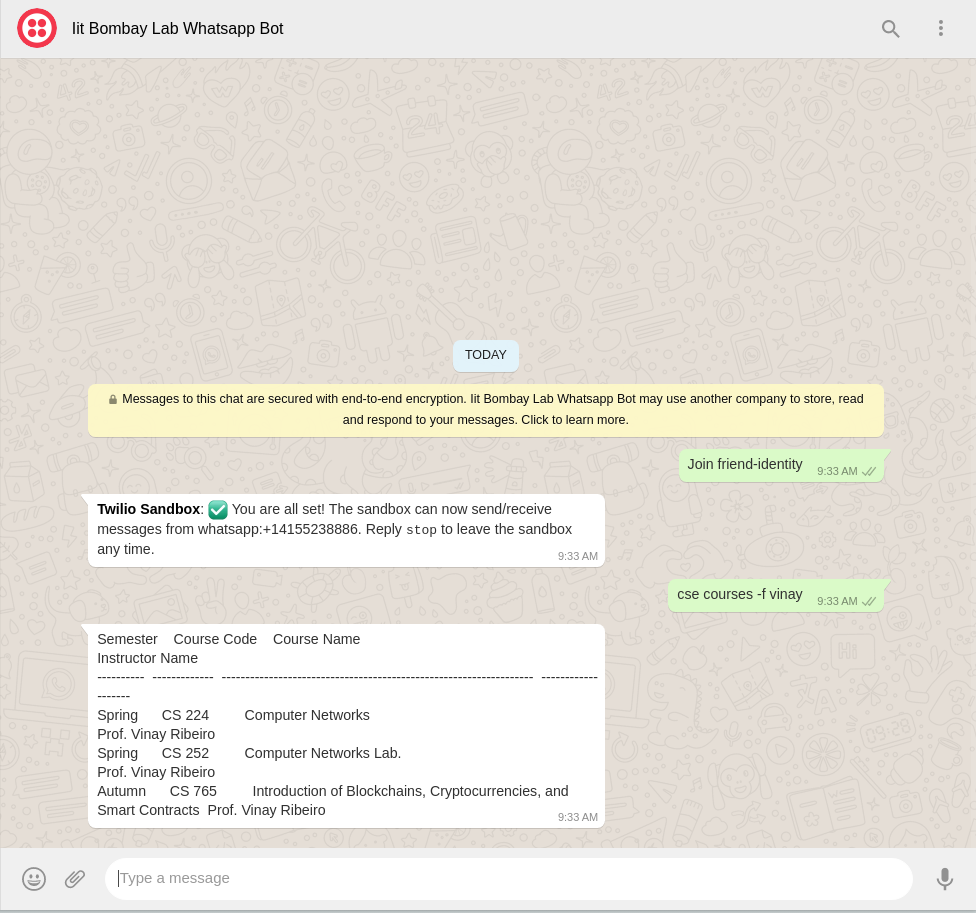
\includegraphics[width=14cm, height=10cm]{whatsappbot}

\section{Future scope}
This project aims at easing the life of a student at IIT-B by gathering most of the things in one place. A student can fetch information directly on command line when he or she is working on something, and does not have to use the UI and go through login procedures that you'd normally have to when fetching information otherwise.\\
The future improvements that can be made are to include fetching information from "Bodhitree", fetch updates from "Microsoft team APIs" and add features to the existing modules, such as getting a list of publications, information on exam timetable, academic timetable and so on.

\end{document}